\documentclass{article}
\usepackage{caption}
\usepackage{subcaption}
\usepackage{graphicx}
\usepackage{tikz}
\usepackage{tikzsymbols}
\usetikzlibrary{calc}
\usepackage{float}
\usepackage{pdflscape}
\usepackage{geometry}
\geometry{a4paper, landscape, margin=1cm}

\def\centerarc[#1](#2)(#3:#4:#5){\draw[#1] ($(#2)+({#5*cos(#3)},{#5*sin(#3)})$) arc (#3:#4:#5);}

\pagestyle{empty}
\begin{document}
	\centering
	\begin{figure}[H]
			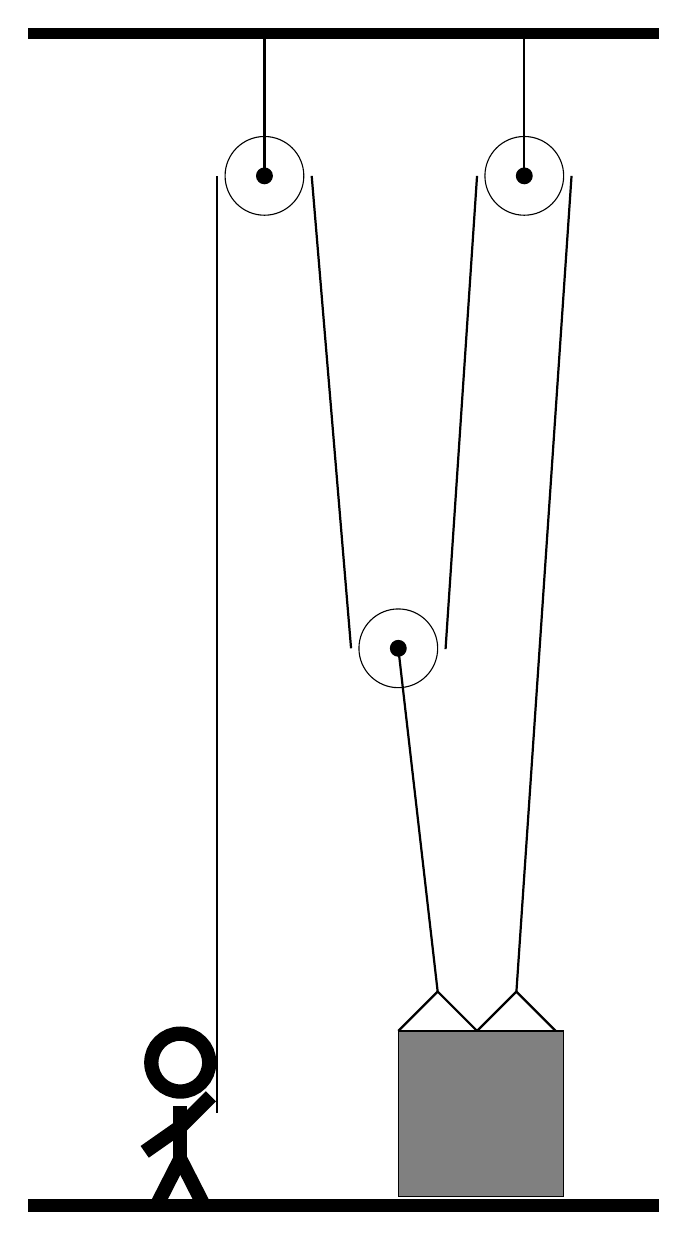
\begin{tikzpicture}
				%%%%% START %%%%%
				\def\a{11.75}
				\def\radlg{0.5}
				\def\radrp{0.6}
				\def\radsm{0.1}
				\def\xone{1}
				\def\yone{10}
				\def\xtwo{4.3}
				\def\ytwo{10}
				\def\xthree{2.7}
				\def\ythree{4}
				\def\xh{3.2}
				\def\hlentwo{10.36}
				\def\hlen{10.36}
				
				\draw[fill=black] (-2,\a) rectangle (6,\a+0.125);

				\draw (\xone,\yone) circle (\radlg);
				\draw[fill=black] (\xone,\yone) circle (\radsm);
				\draw[thick] (\xone,\yone) -- (\xone,\a);

				\draw (\xtwo,\ytwo) circle (\radlg);
				\draw[fill=black] (\xtwo,\ytwo) circle (\radsm);
				\draw[thick] (\xtwo,\ytwo) -- (\xtwo,\a);

				\draw (\xthree,\ythree) circle (\radlg);
				\draw[fill=black] (\xthree,\ythree) circle (\radsm);


				\draw[thick]  (\xh-0.5,\ytwo-\hlentwo-0.5) -- (\xh,\ytwo-\hlentwo) -- (\xh+0.5,\ytwo-\hlentwo-0.5);
				\draw[thick]  (\xh+0.5,\yone-\hlen-0.5) -- (\xh+1,\yone-\hlen) -- (\xh+1.5,\yone-\hlen-0.5);
				\draw[fill=black!50] (\xh-0.5,\yone-\hlen-0.5) rectangle (\xh+1.6,\yone-\hlen-0.5-2.1);
				
				\draw[thick] (\xone-\radrp,-1.9) -- (\xone-\radrp,\yone);
				\centerarc[thick](\xone,\yone)(0:180:\radrp);
				\draw[thick] (\xone+\radrp,\yone) -- (\xthree-\radrp,\ythree);
				\centerarc[thick](\xthree,\ythree)(180:370:\radrp);
				\draw[thick] (\xthree+\radrp,\ythree-0.01) -- (\xtwo-\radrp,\ytwo);
				\centerarc[thick](\xtwo,\ytwo)(0:180:\radrp);
				\draw[thick] (\xh+1,\yone-\hlen) -- (\xtwo+\radrp,\ytwo);
				\draw[thick] (\xh,\yone-\hlen) -- (\xthree,\ythree);

				\node at (-0.1,-2) {\Strichmaxerl[10][35][45]};
						
				\draw[fill=black] (-2,-3) rectangle (6,-3.15);
				%%%%% START %%%%%
			\end{tikzpicture}
	\end{figure}

\end{document}